\chapter{Molecular Plant Physiology and Stress Responses}\label{ch:b3:plant-molecular-physiology}

A bean seedling grown in a dark cupboard is a pale, spindly thing: a
long white stem, a hook at the top, two folded yellow leaves. Move it
to a window and within a day it has stopped elongating, straightened
its hook, spread and greened its leaves --- a different organism, from
the same genes. It had not been waiting for energy; it had been waiting
for information. A red photon absorbed by a single protein tells it
that it has reached the light; the ratio of red to far-red tells it
whether a neighbour's leaf is overhead; the length of the night tells
it the season; a drop in the water potential of its roots, a touch of
wind, the flagellin of a bacterium on its leaf --- each is detected by a
receptor, converted to a chemical signal, and answered by a change in
which genes are expressed and which cells grow. A plant cannot run
from its environment; it must read it and remodel itself. This chapter
is about that reading: the photoreceptors, the \omterm{def:b3:endocrinology:hormone}{hormones} and how they
act at the molecular scale, the responses to drought, salt, cold and
heat, and the two-layered immune system that plants evolved without a
single mobile cell.

\section{Reading the light}

\begin{definition}[Photoreceptors]\label{def:b3:plant-molecular-physiology:photoreceptors}
\index{phytochrome}\index{cryptochrome}\index{phototropin}\index{photomorphogenesis}\index{etiolation}
Plants sense light with three families of proteins, none of them
chlorophyll. \emph{Phytochromes} are dimers with a bilin pigment
switched by red light (\qty{660}{nm}) from the inactive \emph{Pr} form
to the active \emph{Pfr}, and back by far-red (\qty{730}{nm}); Pfr
moves into the nucleus and marks a family of transcription factors, the
PIFs, for degradation, releasing the genes of light-grown development;
in darkness Pfr slowly reverts. \emph{Cryptochromes} (blue,
\qty{450}{nm}) are flavoproteins related to DNA-repair enzymes,
controlling de-etiolation, the clock and flowering; \emph{phototropins}
(blue) are membrane kinases that direct bending toward light, the
opening of stomata and the movement of chloroplasts. A seedling in the
dark is \emph{etiolated} --- long hypocotyl, closed cotyledons, no
chlorophyll, all resources spent on reaching the surface; light
switches it to \emph{photomorphogenesis}, and the switch is thrown by
Pfr and cryptochrome inactivating a single repressor complex (COP1)
that in darkness destroys the transcription factors of the light
programme. Light is thus read twice: as energy, by the chloroplast, and
as signal, by receptors sensitive to photon fluxes a million times
smaller.
\end{definition}

\begin{proposition}[The phytochrome photoequilibrium]\label{prop:b3:plant-molecular-physiology:photoequilibrium}
\index{photoequilibrium}\index{red:far-red ratio}\index{shade avoidance}
Under continuous light Pr and Pfr interconvert until the two
photoconversion rates balance: with $k_{1}$ the rate of Pr $\to$ Pfr
(proportional to the red flux) and $k_{2}$ that of Pfr $\to$ Pr
(proportional to the far-red flux, plus a little from red, which Pfr
also absorbs), the fraction of active form is
\[
\varphi = \frac{[\text{Pfr}]}{[\text{Pfr}] + [\text{Pr}]} = \frac{k_{1}}{k_{1} + k_{2}},
\]
independent of the total flux and set only by the \emph{\omterm{prop:b3:plant-molecular-physiology:photoequilibrium}{red:far-red
ratio}} $\zeta$ of the light. Pure red gives $\varphi \approx 0.87$ (Pfr
absorbs some red too), pure far-red $0.03$; open daylight, $\zeta \approx
1.15$, gives about $0.55$, and the light under a leaf canopy, whose
chlorophyll has taken out the red and let the far-red through, has
$\zeta \approx 0.2$ and $\varphi \approx 0.2$. A plant reads its
$\varphi$ as the presence of neighbours: a low value triggers the
\emph{shade-avoidance} syndrome --- elongated stems, raised leaves,
early flowering, less branching --- through the PIFs that Pfr no longer
destroys. A farmer's dense planting is a race of shade-avoiders; the
dwarf wheats of the Green Revolution, insensitive to the signal, put the
saved growth into grain.
\end{proposition}
\begin{proof}
$\mathrm{d}[\text{Pfr}]/\mathrm{d}t = k_{1}[\text{Pr}] - k_{2}[\text{Pfr}]$
with $[\text{Pr}] + [\text{Pfr}] = P$ fixed gives, at steady state,
$k_{1}(P - [\text{Pfr}]) = k_{2}[\text{Pfr}]$, whence $\varphi = k_{1}/
(k_{1} + k_{2})$. Both rates are proportional to the incident flux, so
scaling the light scales both and leaves $\varphi$ unchanged; only the
spectral composition matters. The steady state is approached with rate
$k_{1} + k_{2}$ --- seconds in sunlight, minutes at dusk --- and the
dark reversion of Pfr, with a half-life of hours, sets what remains at
night.
\end{proof}

\begin{omfigure}
\begin{tikzpicture}[every node/.style={font=\scriptsize}, >=stealth]
  \node[draw, very thick, omDef, fill=omDef!15, rounded corners, minimum width=1.6cm, minimum height=0.9cm] (pr) at (0,0) {Pr (inactive)};
  \node[draw, very thick, omThm, fill=omThm!15, rounded corners, minimum width=1.6cm, minimum height=0.9cm] (pfr) at (4.2,0) {Pfr (active)};
  \draw[->, very thick, red!70!black] (pr.north east) to[bend left=25] node[above] {red, \qty{660}{nm}} (pfr.north west);
  \draw[->, very thick, red!40!black] (pfr.south west) to[bend left=25] node[below] {far-red, \qty{730}{nm}} (pr.south east);
  \draw[->, thick, gray] (pfr.south) ++(0.5,-0.15) to[bend left=40] node[right, font=\tiny, gray] {dark reversion, hours} ++(-0.3,-0.9);
  \draw[->, thick] (pfr.east) -- ++(1.0,0) node[right, align=left] {into the nucleus:\\PIFs degraded, COP1 off;\\light-grown programme on};
  \begin{scope}[shift={(0,-4.6)}]
  \begin{axis}[
    width=0.55\linewidth, height=4.6cm,
    axis x line=bottom, axis y line=left,
    xmin=0, xmax=2.5, ymin=0, ymax=1,
    xlabel={red:far-red ratio $\zeta$}, ylabel={$\varphi = $ Pfr fraction},
    xlabel style={font=\scriptsize, at={(axis description cs:0.5,-0.15)}, anchor=north}, ylabel style={font=\scriptsize},
    tick label style={font=\scriptsize}, xtick={0.2,0.5,1.15,2}, xticklabels={0.2,0.5,1.15,2}, ytick={0.2,0.55,0.87},
    clip=false,
  ]
  \addplot[very thick, omDef, domain=0:2.5, samples=80] {0.87*x/(x+0.6)};
  \draw[dashed, gray] (axis cs:0.2,0) -- (axis cs:0.2,0.22) -- (axis cs:0,0.22);
  \draw[dashed, gray] (axis cs:1.15,0) -- (axis cs:1.15,0.57) -- (axis cs:0,0.57);
  \node[font=\tiny, anchor=west, align=left] at (axis cs:0.25,0.12) {under a canopy:\\shade avoidance};
  \node[font=\tiny, anchor=south west] at (axis cs:1.2,0.62) {open daylight};
  \node[font=\tiny, anchor=north west, omDef, align=left] at (axis cs:1.6,0.45) {an empirical fit,\\$\varphi \approx 0.87\,\zeta/(\zeta + 0.6)$};
  \end{axis}
  \end{scope}
\end{tikzpicture}

{\small The \omterm{def:b3:plant-molecular-physiology:photoreceptors}{phytochrome} switch. Red light makes the active form,
far-red unmakes it, darkness slowly reverts it; the steady fraction of
active form depends on the colour balance of the light and not on its
brightness, which is how a seedling knows a leaf is above it.}
\end{omfigure}

\begin{proof}[Evidence]
Borthwick, Hendricks and colleagues (1952) gave lettuce seeds brief
flashes: red made them germinate, far-red given afterwards cancelled it,
red again restored it, and so on through a dozen alternations --- the
last flash decided, the signature of a reversible pigment, which they
then extracted (1959) as a blue protein that changed its absorption
spectrum under red and far-red. The dark-grown seedling's whole
programme was later shown to hang on one repressor: mutants lacking
COP1 develop in total darkness as if in light, short and green-ready,
and phytochrome- and cryptochrome-deficient mutants stay etiolated in
the light.
\end{proof}

\begin{omfigure}
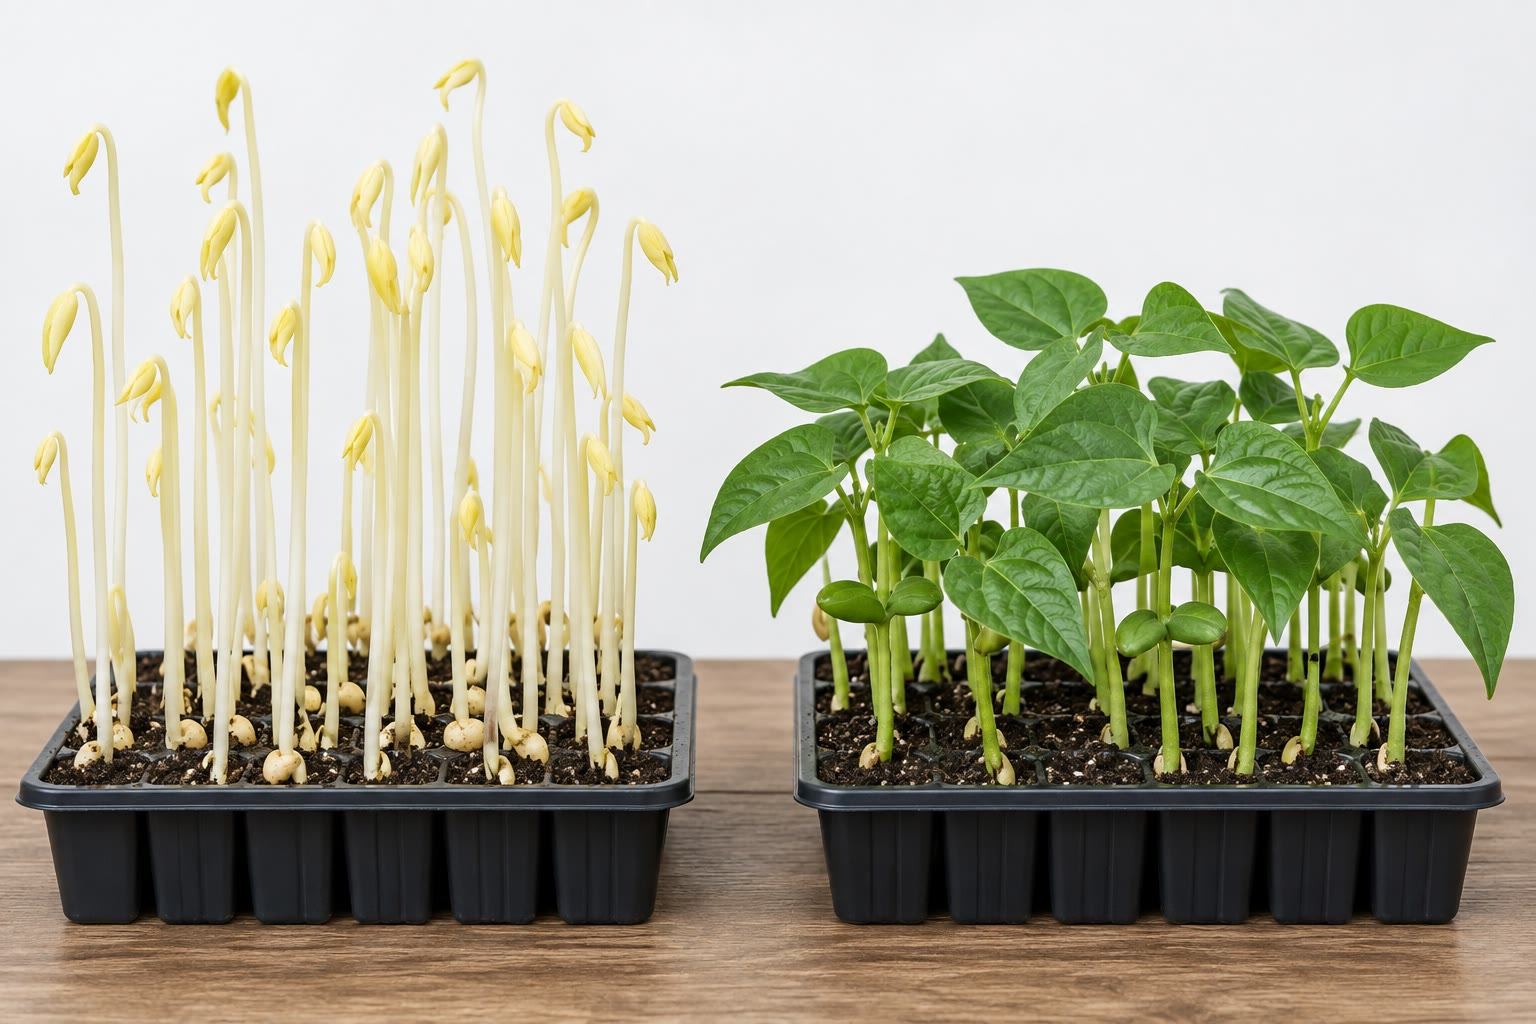
\includegraphics[width=0.56\linewidth]{images/book5/ai/b5-22-etiolated-seedlings.jpg}

{\small Seedlings grown in darkness and in light: the same genome,
two developmental programmes, and the difference is a single red photon
absorbed by \omterm{def:b3:plant-molecular-physiology:photoreceptors}{phytochrome}.}
\end{omfigure}

\section{Hormones at the molecular scale}

\begin{definition}[The plant hormones and their receptors]\label{def:b3:plant-molecular-physiology:hormones}
\index{auxin}\index{TIR1}\index{gibberellin}\index{DELLA}\index{abscisic acid}\index{ethylene}\index{cytokinin}\index{brassinosteroid}
The Year~1 volume described what the plant \omterm{def:b3:endocrinology:hormone}{hormones} do; here is how
they are heard. Several act by \emph{regulated destruction}.
\emph{Auxin} (indole-3-acetic acid) binds the F-box protein
\emph{TIR1}, gluing it to the Aux/IAA repressors, which are then
ubiquitinated and destroyed by the proteasome: the auxin-response genes
they were repressing switch on within minutes --- the \omterm{def:b3:endocrinology:hormone}{hormone} is a
molecular glue, and the receptor is part of the degradation machinery.
\emph{Gibberellin} does the same with the \emph{DELLA} repressors of
growth, through its receptor GID1: the dwarf wheats and rices of the
Green Revolution carry DELLA proteins that cannot be destroyed, and so
stay short however much gibberellin they make. \emph{Jasmonate}
follows the same logic with the JAZ repressors. \emph{Abscisic acid}
(ABA), the \omterm{def:b3:endocrinology:hormone}{hormone} of drought and dormancy, binds the PYR/PYL
receptors, which then inhibit a phosphatase (PP2C), releasing a kinase
(SnRK2) that phosphorylates ion channels and transcription factors ---
a double negative that makes the response steep. \emph{Ethylene}, a
gas, binds copper-containing receptors in the ER membrane that in its
absence actively repress the response; binding switches them off, and
the ripening, \omterm{def:b3:cell-cycle-apoptosis:other}{senescence} and stress genes come on. \emph{Cytokinins}
act through histidine-kinase receptors like bacterial \omterm{def:b3:bacteriology:quorum}{two-component
systems}; \emph{brassinosteroids}, the plant's steroids, through a
surface receptor kinase, not a \omterm{def:b3:endocrinology:hormone}{nuclear receptor} --- the only \omterm{def:b3:endocrinology:hormone}{steroid
hormones} anywhere heard at the cell surface. Plants have no glands: each
\omterm{def:b3:endocrinology:hormone}{hormone} is made where it is needed, or moved by specific carriers, and
its concentration is set locally by synthesis, conjugation and
destruction.
\end{definition}

\begin{theorem}[Chemiosmotic polar transport of auxin]\label{thm:b3:plant-molecular-physiology:auxin}
\index{polar auxin transport}\index{PIN proteins}\index{anion trapping}
Indole-3-acetic acid is a weak acid, $\mathrm{p}K_{a} = 4.75$. In the
cell wall space at pH~$5.5$ a substantial fraction is the neutral
IAAH, which diffuses across the membrane; in the cytosol at pH~$7.2$
nearly all is the anion IAA$^{-}$, which cannot leave by diffusion. At
equilibrium of the neutral form across the membrane the ratio of total
\omterm{def:b3:plant-molecular-physiology:hormones}{auxin} inside to outside is
\[
\frac{[\text{IAA}]_{\text{in}}}{[\text{IAA}]_{\text{out}}}
= \frac{1 + 10^{\,\mathrm{pH}_{\text{in}} - \mathrm{p}K_{a}}}{1 + 10^{\,\mathrm{pH}_{\text{out}} - \mathrm{p}K_{a}}}
\approx \frac{283}{6.6} \approx 43 :
\]
the cell traps \omterm{def:b3:plant-molecular-physiology:hormones}{auxin} forty-fold. It can leave only through the
\emph{PIN} efflux carriers, and because each cell places its PINs on one
face --- the basal face in the stem --- the \omterm{def:b3:plant-molecular-physiology:hormones}{auxin} taken up all round
leaves at the bottom, enters the next cell, and so on: a column of
cells with the same polarity is a conveyor moving \omterm{def:b3:plant-molecular-physiology:hormones}{auxin} at about
\qty{1}{cm/h} from shoot tip to root, and re-orienting the PINs
re-directs the stream, which is how a shaded side of a stem comes to
hold more \omterm{def:b3:plant-molecular-physiology:hormones}{auxin} and grow faster.
\end{theorem}
\begin{proof}
Henderson--Hasselbalch: $[\text{IAA}^{-}]/[\text{IAAH}] = 10^{\,\mathrm{pH}
- \mathrm{p}K_{a}}$, so total $= [\text{IAAH}](1 + 10^{\,\mathrm{pH} -
\mathrm{p}K_{a}})$. The neutral form equilibrates, $[\text{IAAH}]_{\text{in}}
= [\text{IAAH}]_{\text{out}}$; dividing the totals gives the ratio,
$(1 + 10^{2.45})/(1 + 10^{0.75}) = 283/6.6$. With PINs on one face,
the anion's only exit is directional; a column of $n$ cells passes the
flux along, and the measured velocity, an order of magnitude above
diffusion over these distances, is that of carrier-mediated efflux at
each cell boundary. The Cholodny--Went hypothesis (1920s) that bending
follows a lateral redistribution of \omterm{def:b3:plant-molecular-physiology:hormones}{auxin} was confirmed by direct
measurement in oat coleoptiles and by imaging PIN relocation in
\emph{Arabidopsis} roots turned on their side (2000s).
\end{proof}

\begin{omfigure}
\begin{tikzpicture}[every node/.style={font=\scriptsize}, >=stealth]
  % three cells in a column
  \foreach \y in {0,-2.2,-4.4} {
    \draw[thick, omDef, fill=omDef!8] (0,\y) rectangle (3.2,\y-1.9);
    \draw[very thick, omThm] (0.6,\y-1.9) -- (2.6,\y-1.9);
    \node[right, font=\tiny] at (3.3,\y-0.4) {cytosol pH 7.2};
    \node[right, font=\tiny] at (3.3,\y-0.8) {IAA$^{-}$ trapped};
    \draw[->, thick, omDef!70!black] (-0.6,\y-0.6) -- (0.4,\y-0.6); \node[left, font=\tiny] at (-0.6,\y-0.6) {IAAH in};
    \draw[->, thick, omDef!70!black] (3.8,\y-1.3) -- (2.8,\y-1.3);
    \draw[->, very thick, omThm] (1.6,\y-1.5) -- (1.6,\y-2.35);
  }
  \node[left, align=right, font=\tiny] at (-0.6,-1.4) {wall pH 5.5:\\\qty{15}{\%} IAAH,\\\qty{85}{\%} IAA$^{-}$};
  \node[omThm, right, font=\tiny] at (3.3,-2.05) {PIN efflux carriers, basal face only};
  \node[above] at (1.6,0.1) {shoot tip: auxin source};
  \node[below] at (1.6,-6.8) {toward the root, \qty{1}{cm/h}};
  \node[right, align=left] at (5.4,-3.6) {inside : outside $\approx 43 : 1$\\(trapping of the anion)\\[3pt]exit only through PINs,\\so the column is a conveyor;\\move the PINs to a side face\\and the stream turns};
\end{tikzpicture}

{\small The chemiosmotic model of \omterm{thm:b3:plant-molecular-physiology:auxin}{polar auxin transport}. The acid enters
any face as the neutral molecule, is trapped as the anion at the
cytosol's pH, and leaves only through carriers the cell has placed on
one face --- so a file of cells passes \omterm{def:b3:plant-molecular-physiology:hormones}{auxin} in one direction.}
\end{omfigure}

\begin{example}[Gravitropism and phototropism]\label{ex:b3:plant-molecular-physiology:tropism}
Turn a seedling on its side. In the root cap, dense starch-filled
plastids settle onto the new lower side of the columella cells within
minutes; the PIN3 carriers of those cells relocate to the lower face;
\omterm{def:b3:plant-molecular-physiology:hormones}{auxin} flows preferentially down the lower flank of the root, where,
above the optimum for root cells, it \emph{inhibits} elongation, and
the root curves downward. In the shoot the same lateral flow to the
lower side \emph{promotes} elongation (shoot cells' optimum is higher),
and the shoot curves upward. Phototropism: \omterm{def:b3:plant-molecular-physiology:photoreceptors}{phototropin} on the lit side
of a shoot alters PIN placement so that \omterm{def:b3:plant-molecular-physiology:hormones}{auxin} accumulates on the shaded
side, which grows faster, bending the shoot toward the light. Both
movements are slow --- hours --- because they are growth, not motion,
and both are irreversible in the tissue that has grown. Darwin (1880)
showed the tip of a grass seedling perceives the light and the region
below bends; Went (1928) collected the influence in an agar block placed
on a cut tip and showed a block placed asymmetrically on a decapitated
shoot made it bend: the influence was a diffusible substance, which
was then named \omterm{def:b3:plant-molecular-physiology:hormones}{auxin}.
\end{example}

\section{Water, salt, cold and heat}

\begin{definition}[Abiotic stress]\label{def:b3:plant-molecular-physiology:abiotic}
\index{drought stress}\index{osmotic adjustment}\index{salt stress}\index{cold acclimation}\index{heat shock proteins}
A plant cannot escape, so it hardens. \emph{Drought}: falling water
potential in the roots triggers ABA synthesis; ABA closes stomata within
minutes, and over days switches on genes for \emph{osmotic adjustment}
(proline, sugars and other compatible solutes accumulate, lowering the
cell's water potential so it keeps drawing water), for dehydrins that
protect proteins, and for a smaller leaf area and a deeper root.
\emph{Salt} is drought plus poison: sodium enters through potassium
channels and competes with potassium; tolerant plants pump it back out
of roots (the SOS pathway), into vacuoles (NHX exchangers), or excrete it
from leaf glands, and their \emph{halophyte} extreme lives in sea water.
\emph{Cold}: chilling stiffens membranes and slows enzymes; freezing
draws water from cells into extracellular ice and desiccates them.
\emph{Cold acclimation} --- a week of cool days --- induces the CBF
transcription factors, which turn on hundreds of genes for
membrane-fluidising lipids, sugars, antifreeze proteins and dehydrins,
and a winter rye that would die at \qty{-5}{\celsius} in August survives
\qty{-30}{\celsius} in January. \emph{Heat} unfolds proteins; within
minutes of a rise a heat-shock factor releases \emph{heat-shock
proteins}, \omterm{def:b3:structural-biology:chaperones}{chaperones} that refold or dispose of them, the same families
as in every organism. \emph{Flooding} starves roots of oxygen;
rice makes air channels (aerenchyma) and elongates to keep its leaves
above water, \omterm{def:b3:plant-molecular-physiology:hormones}{ethylene} being the signal that accumulates when it cannot
escape into the water. Many of these programmes overlap --- ABA, reactive
oxygen species and calcium spikes are shared second messengers --- and a
plant acclimated to one stress is often partly protected against
another.
\end{definition}

\begin{proposition}[The stoma as a valve]\label{prop:b3:plant-molecular-physiology:stomata}
\index{stoma}\index{guard cell}\index{stomatal conductance}\index{water-use efficiency}
A pair of \emph{\omterm{prop:b3:plant-molecular-physiology:stomata}{guard cells}} bounds each stomatal pore; the pore opens
when they take up potassium and anions (and make sugar), swell, and
bow apart, and closes when they lose them. Blue light (\omterm{def:b3:plant-molecular-physiology:photoreceptors}{phototropins}),
low CO$_{2}$ and humidity open; darkness, high CO$_{2}$, drought and
ABA close. ABA's route: receptor $\to$ phosphatase inhibited $\to$
kinase active $\to$ anion channels (SLAC1) open $\to$ the membrane
depolarises $\to$ potassium leaves through outward channels $\to$ water
follows $\to$ the pore shuts, in ten minutes. The pore is where the
plant's central trade is made: CO$_{2}$ diffuses in and water vapour
out through the same hole, and because the vapour gradient (a leaf at
\qty{100}{\%} humidity inside against air at \qty{50}{\%}) is fifty
times steeper than the CO$_{2}$ gradient (\qty{400}{ppm} outside,
\qty{250}{} inside), a leaf loses several hundred molecules of water
for every molecule of carbon it fixes. The \emph{\omterm{prop:b3:plant-molecular-physiology:stomata}{stomatal conductance}}
$g_{s}$ sets both fluxes: transpiration $E = g_{s}\,\Delta w$ and
assimilation $A = (g_{s}/1.6)\,\Delta c$ (CO$_{2}$ being heavier, it
diffuses $1.6$ times more slowly), so the \emph{\omterm{prop:b3:plant-molecular-physiology:stomata}{water-use efficiency}}
$A/E = \Delta c/(1.6\,\Delta w)$ depends on the gradients, not on how
far the pore is open; closing the pore lowers both fluxes together, and
raising the internal CO$_{2}$ (C$_{4}$ plants, which concentrate it) or
opening only at night (CAM plants, in cool humid air) is how desert
plants improve the ratio.
\end{proposition}
\begin{proof}
Fick's law across the pore for each gas, with the same geometric
conductance scaled by the ratio of diffusion coefficients
$D_{\mathrm{H_2O}}/D_{\mathrm{CO_2}} = 1.6$; dividing the two fluxes
cancels $g_{s}$. Numbers: $\Delta w \approx \qty{15}{mmol/mol}$ of air
at \qty{25}{\celsius} and \qty{50}{\%} humidity, $\Delta c \approx
\qty{150}{\micro mol/mol}$: $A/E = 150/(1.6\times\num{15000}) = 1/160$
--- $160$ water molecules per CO$_{2}$ under those mild conditions,
$500$ in dry air. The sequence of ABA's action was worked out with
guard-cell protoplasts under patch clamp, the anion current appearing
within a minute of ABA and the mutant lacking SLAC1 failing to close.
\end{proof}

\begin{omfigure}
\begin{tikzpicture}[every node/.style={font=\scriptsize}, >=stealth]
  % pore with two guard cells
  \begin{scope}[shift={(0,0)}]
    \fill[omProp!30] (0,0) ellipse (1.4 and 0.9);
    \fill[white] (0,0) ellipse (0.5 and 0.6);
    \draw[thick, omProp!80!black] (0,0) ellipse (1.4 and 0.9); \draw[thick, omProp!80!black] (0,0) ellipse (0.5 and 0.6);
    \node[below, font=\tiny] at (0,-1.0) {open: K$^{+}$, Cl$^{-}$, malate in, turgid};
    \draw[->, thick, omDef] (0,0.3) -- (0,1.5) node[above, font=\tiny] {H$_2$O out, $E = g_{s}\Delta w$};
    \draw[->, thick, omThm] (0,1.5) ++(-1.0,0) -- ++(0,-1.2); \node[left, font=\tiny, omThm] at (-1.1,1.0) {CO$_2$ in, $A = g_{s}\Delta c/1.6$};
  \end{scope}
  \begin{scope}[shift={(4.2,0)}]
    \fill[omProp!30] (0,0) ellipse (1.2 and 0.75);
    \draw[thick, omProp!80!black] (0,0) ellipse (1.2 and 0.75); \draw[very thick, omProp!80!black] (0,-0.5) -- (0,0.5);
    \node[below, font=\tiny] at (0,-0.9) {closed: ions lost, flaccid};
  \end{scope}
  \draw[->, thick] (1.6,0) -- (2.8,0) node[midway, above, font=\tiny] {ABA, dark,};
  \node[font=\tiny] at (2.2,-0.25) {high CO$_2$};
  % ABA pathway chain
  \begin{scope}[shift={(7.0,1.7)}]
    \node[draw, rounded corners, fill=omDef!20, align=center, font=\tiny] (a) at (0,0) {ABA binds\\PYR/PYL};
    \node[draw, rounded corners, fill=omThm!15, align=center, font=\tiny] (b) at (0,-0.9) {PP2C phosphatase\\inhibited};
    \node[draw, rounded corners, fill=omMeth!25, align=center, font=\tiny] (c) at (0,-1.8) {SnRK2 kinase\\active};
    \node[draw, rounded corners, fill=omProp!25, align=center, font=\tiny] (d) at (0,-2.7) {SLAC1 anion channel\\open: depolarisation};
    \node[draw, rounded corners, fill=omProp!25, align=center, font=\tiny] (e) at (0,-3.6) {K$^{+}$ out, water out,\\pore shuts in \qty{10}{min}};
    \draw[-|, thick] (a) -- (b); \draw[-|, thick] (b) -- (c); \draw[->, thick] (c) -- (d); \draw[->, thick] (d) -- (e);
    \node[right, font=\tiny, align=left] at (1.5,-0.9) {two inhibitions\\in series:\\a steep switch};
  \end{scope}
\end{tikzpicture}

{\small The stoma and the signal that shuts it. Water and carbon dioxide
share the pore, so the plant trades one for the other at a rate set by
the two gradients; drought's \omterm{def:b3:endocrinology:hormone}{hormone} closes the valve through a chain
of two inhibitions, which makes the response switch-like.}
\end{omfigure}

\begin{omfigure}
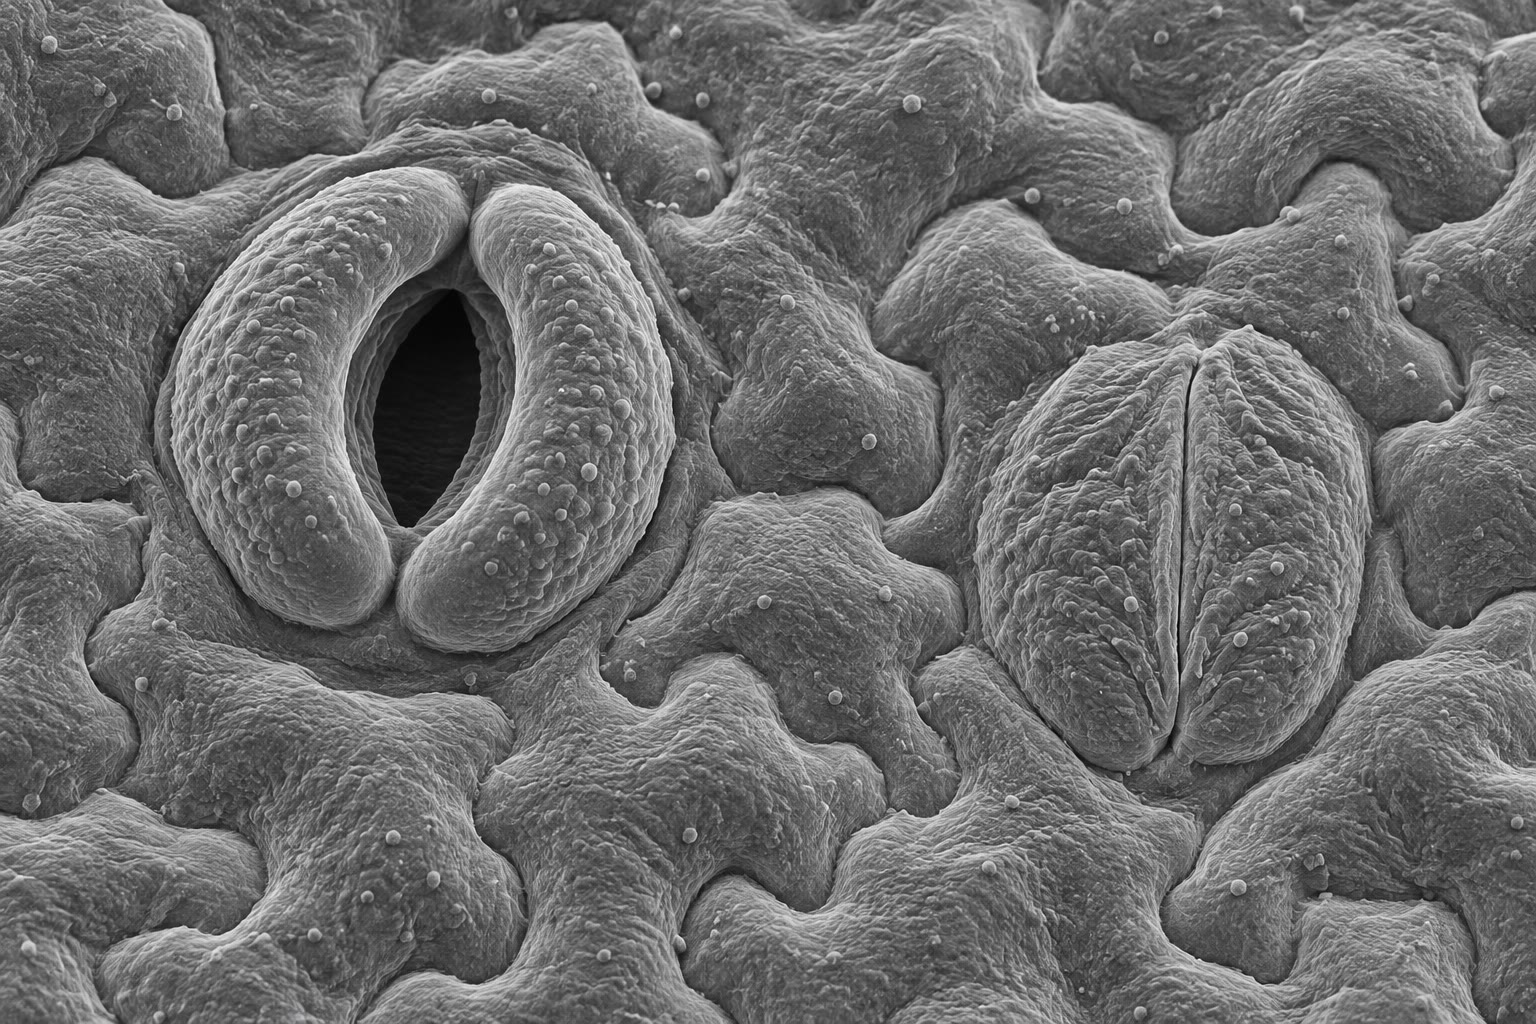
\includegraphics[width=0.46\linewidth]{images/book5/ai/b5-22-stomata-sem.jpg}\hspace{0.04\linewidth}
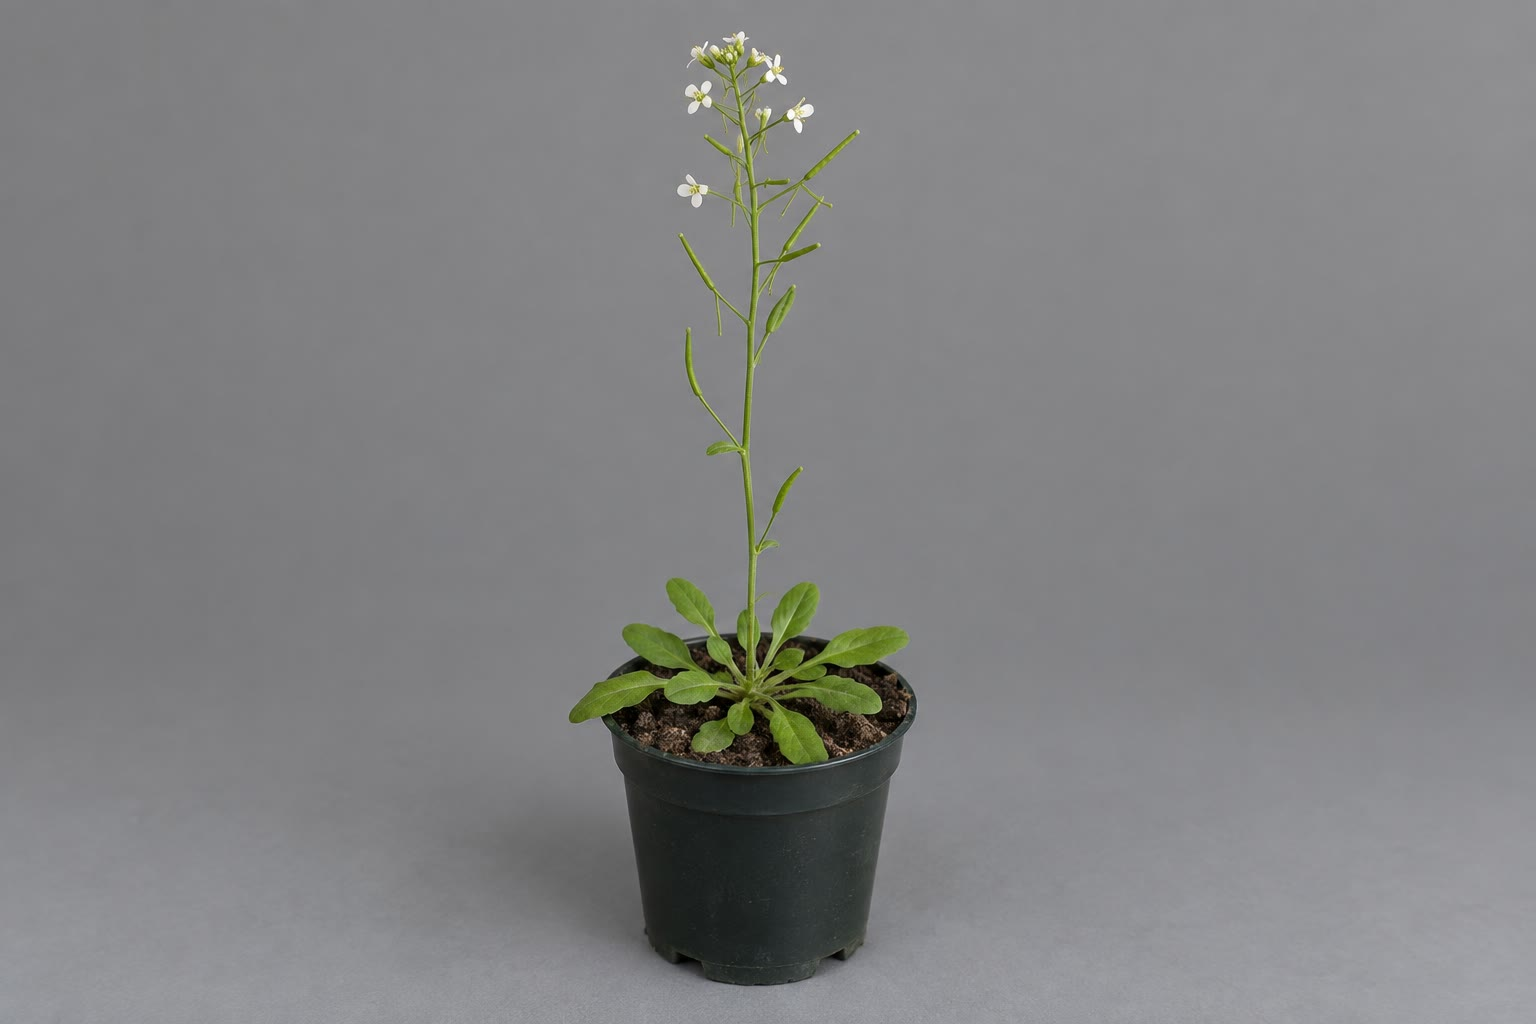
\includegraphics[width=0.46\linewidth]{images/book5/ai/b5-22-arabidopsis.jpg}

{\small Left: stomata on a leaf surface, each pore between its two
\omterm{prop:b3:plant-molecular-physiology:stomata}{guard cells}, some open and some closed. Right: \emph{Arabidopsis
thaliana}, a roadside weed with a small genome, a six-week generation and
a hundred thousand mutant lines, in which most of this chapter's
molecules were found.}
\end{omfigure}

\section{Immunity without immune cells}

\begin{definition}[Two layers of plant immunity]\label{def:b3:plant-molecular-physiology:immunity}
\index{pattern-triggered immunity}\index{effector-triggered immunity}\index{NLR receptor}\index{hypersensitive response}\index{systemic acquired resistance}\index{salicylic acid}\index{jasmonic acid}
Every plant cell is its own immune cell. The first layer,
\emph{pattern-triggered immunity} (PTI), uses surface receptor kinases
that recognise molecules common to whole classes of microbes ---
FLS2 binds a 22-amino-acid piece of bacterial flagellin, others bind
chitin fragments of fungal walls --- and within minutes launches
calcium influx, a burst of reactive oxygen, kinase cascades, stomatal
closure, wall thickening with callose, and the transcription of hundreds
of defence genes; it holds off most microbes. Pathogens that succeed
inject \emph{effectors} --- proteins that disable PTI components --- and
against these the second layer, \emph{effector-triggered immunity}
(ETI), fields intracellular \emph{NLR receptors} (nucleotide-binding,
leucine-rich repeat), each recognising one effector or the damage it
does, in the gene-for-gene pairing Flor described in flax rust
(1940s). ETI is faster and stronger than PTI and usually ends in the
\emph{hypersensitive response}: the infected cell and its neighbours
kill themselves, walling the pathogen in dead tissue --- the small brown
flecks on a resistant leaf. Both layers release \omterm{def:b3:endocrinology:hormone}{hormones} that carry the
alarm: \emph{salicylic acid} against biotrophs (which feed on living
cells), triggering \emph{systemic acquired resistance} throughout the
plant for weeks; \emph{jasmonic acid} and \omterm{def:b3:plant-molecular-physiology:hormones}{ethylene} against necrotrophs
(which kill and then feed) and chewing insects, with volatile
jasmonates warning neighbouring plants and attracting the insects'
parasitoids. The two \omterm{def:b3:endocrinology:hormone}{hormones} antagonise each other, and some pathogens
exploit it: a bacterium that makes a jasmonate mimic switches off the
salicylate defence that would have stopped it.
\end{definition}

\begin{omfigure}
\begin{tikzpicture}
\begin{axis}[
  width=0.78\linewidth, height=5.4cm,
  axis x line=bottom, axis y line=left,
  xmin=0, xmax=10, ymin=0, ymax=10,
  xlabel={the arms race, from left to right}, ylabel={amplitude of defence},
  xlabel style={font=\small, at={(axis description cs:0.5,-0.08)}, anchor=north}, ylabel style={font=\small},
  xtick=\empty, ytick=\empty,
  clip=false,
]
\addplot[very thick, omDef] coordinates {(0,1) (1.5,5)};
\addplot[very thick, omThm] coordinates {(1.5,5) (3.2,1.8)};
\addplot[very thick, omDef] coordinates {(3.2,1.8) (4.8,8)};
\addplot[very thick, omThm] coordinates {(4.8,8) (6.4,2.2)};
\addplot[very thick, omDef] coordinates {(6.4,2.2) (8.0,8.6)};
\draw[dashed, gray] (axis cs:0,4) -- (axis cs:8.5,4); \node[font=\scriptsize, gray, anchor=west] at (axis cs:8.5,4) {resistance threshold};
\draw[dashed, gray] (axis cs:0,7.2) -- (axis cs:8.5,7.2); \node[font=\scriptsize, gray, anchor=west] at (axis cs:8.5,7.2) {hypersensitive response};
\node[font=\scriptsize, omDef, anchor=south west] at (axis cs:0.1,5.3) {PTI: receptors see flagellin, chitin};
\node[font=\scriptsize, omThm, anchor=north, align=center] at (axis cs:3.2,1.6) {effectors injected:\\PTI disabled};
\node[font=\scriptsize, omDef, anchor=south, align=center] at (axis cs:4.8,8.2) {ETI: an NLR recognises\\an effector};
\node[font=\scriptsize, omThm, anchor=north, align=center] at (axis cs:6.4,2.0) {effector lost or altered:\\recognition escaped};
\node[font=\scriptsize, omDef, anchor=south, align=center] at (axis cs:8.0,8.8) {a new NLR\\evolves};
\end{axis}
\end{tikzpicture}

{\small The zigzag of plant--pathogen coevolution. Surface receptors
raise a defence against common microbial molecules; pathogens inject
effectors that suppress it; plants evolve intracellular receptors for
the effectors; pathogens shed or alter them; and so on, each step
leaving genes for resistance and virulence that breeders and pathogens
still trade.}
\end{omfigure}

\begin{proof}[Evidence]
Flor (1940s) crossed flax varieties and rust strains and found that
resistance to each strain segregated as a single dominant plant gene
matched by a single avirulence gene in the fungus --- the gene-for-gene
relation, unexplained for fifty years until the first NLR genes were
cloned (1994) and the first effector--receptor pairs shown to bind or to
mark each other's damage. Gómez-Gómez and Boller (2000) found the
\emph{Arabidopsis} mutant blind to flagellin, \emph{fls2}, and showed
its receptor kinase bound the peptide flg22 at nanomolar concentration
and that the mutant was more susceptible to bacteria sprayed on its
leaves but not to bacteria injected into them --- the receptor guards the
surface and the stomata through which bacteria enter. Ross (1961)
inoculated one leaf of a tobacco plant with a \omterm{def:b3:virology:virus}{virus} and found the other
leaves resistant a week later: \omterm{def:b3:plant-molecular-physiology:immunity}{systemic acquired resistance}, later shown
to need \omterm{def:b3:plant-molecular-physiology:immunity}{salicylic acid}, which the plant makes from the same pathway as
aspirin's parent.
\end{proof}

\begin{example}[The plant clock and the length of the day]\label{ex:b3:plant-molecular-physiology:clock}
Plants keep a \omterm{def:b3:endocrinology:clock}{circadian clock} of the same design as the animal one and
of unrelated parts: morning factors (CCA1, LHY) repress an evening gene
(TOC1) whose product represses them, with further loops that make a
robust 24-hour cycle even in constant light, anticipating dawn by
opening stomata and switching on photosynthesis genes an hour before
the sun. The clock's most consequential output is the measurement of
day length. In \emph{Arabidopsis}, a long-day plant, the clock makes the
CONSTANS protein accumulate in the late afternoon; in a long day that
afternoon is still lit, \omterm{def:b3:plant-molecular-physiology:photoreceptors}{phytochrome} and \omterm{def:b3:plant-molecular-physiology:photoreceptors}{cryptochrome} stabilise the
protein, and it switches on \emph{FT} in the leaf; in a short day the
protein is made in darkness and destroyed. FT protein, the florigen
that grafting experiments had chased since Chailakhyan (1936), travels
in the phloem to the shoot apex and, with a partner there, converts the
apex from making leaves to making flowers. Short-day plants (rice,
soybean) use the same clock with the sign reversed. A plant thus reads
the calendar by comparing an internal rhythm with the external light ---
the ``external coincidence'' that B{\"u}nning proposed in 1936 and that
molecular genetics made literal seventy years later.
\end{example}

\begin{remark}[Standing still, changing everything]\label{rem:b3:plant-molecular-physiology:remark}
The animal's answer to a bad environment is to leave it; the plant's is
to become a different plant. It has receptors for the colour and
direction of light, the pull of gravity, the water potential of its
soil, the touch of wind and the chemistry of its enemies; its \omterm{def:b3:endocrinology:hormone}{hormones}
act by destroying repressors, so that a signal can switch a programme
in minutes; and its every cell is its own sensor, immune system and,
if need be, its own regenerating meristem. The dwarf wheats that fed a
growing world were a \omterm{def:b3:plant-molecular-physiology:hormones}{DELLA} protein that could not be degraded; the
drought-tolerant crops of the next decades will be, in large part, a
matter of ABA receptors, \omterm{prop:b3:plant-molecular-physiology:stomata}{stomatal conductance} and the \omterm{prop:b3:plant-molecular-physiology:stomata}{water-use
efficiency} this chapter has computed.
\end{remark}

\section{Exercises}

\begin{exercise}[$\star$]\label{exo:b3:plant-molecular-physiology:1}
List the three photoreceptor families with their wavelengths and one
response each. Why does a plant need photoreceptors when it already has
chlorophyll?
\end{exercise}

\begin{exercise}[$\star$]\label{exo:b3:plant-molecular-physiology:2}
Explain how \omterm{def:b3:plant-molecular-physiology:hormones}{auxin}, \omterm{def:b3:plant-molecular-physiology:hormones}{gibberellin} and jasmonate share a mechanism of
action, and why this makes the response fast.
\end{exercise}

\begin{exercise}[$\star$]\label{exo:b3:plant-molecular-physiology:3}
Describe the sequence of events from ABA arriving at a \omterm{prop:b3:plant-molecular-physiology:stomata}{guard cell} to
the pore closing, and name the point at which a mutation would leave
the plant unable to close its stomata.
\end{exercise}

\begin{exercise}[$\star$]\label{exo:b3:plant-molecular-physiology:4}
Distinguish pattern-triggered and \omterm{def:b3:plant-molecular-physiology:immunity}{effector-triggered immunity} by what
is recognised, where the receptor is, and how the response ends.
\end{exercise}

\begin{exercise}[$\star\star$]\label{exo:b3:plant-molecular-physiology:5}
Using the fit $\varphi \approx 0.87\,\zeta/(\zeta + 0.6)$, compute the
Pfr fraction in daylight ($\zeta = 1.15$), under one leaf ($\zeta =
0.4$), under a dense canopy ($\zeta = 0.1$), and under an incandescent
lamp ($\zeta = 0.7$). Why do seedlings under such lamps grow tall?
\end{exercise}

\begin{exercise}[$\star\star$]\label{exo:b3:plant-molecular-physiology:6}
Compute the inside:outside ratio for \omterm{def:b3:plant-molecular-physiology:hormones}{auxin} if the wall pH is $5.0$ and
the cytosol $7.5$; then if the wall is acidified to $4.5$ (as growing
cells do). What happens to trapping if the cytosol acidifies to $6.5$
under anoxia?
\end{exercise}

\begin{exercise}[$\star\star$]\label{exo:b3:plant-molecular-physiology:7}
\omterm{def:b3:plant-molecular-physiology:hormones}{Auxin} moves at \qty{1}{cm/h} through cells \qty{50}{\micro m} long. How
many cells does it cross per hour, and how long does it spend in each?
Compare with the time to diffuse \qty{50}{\micro m} ($D =
\qty{5e-10}{m^2/s}$, $t \approx x^{2}/2D$) and say which step limits
the transport.
\end{exercise}

\begin{exercise}[$\star\star$]\label{exo:b3:plant-molecular-physiology:8}
A leaf at \qty{25}{\celsius} has an internal vapour mole fraction of
\qty{32}{mmol/mol} and the air \qty{16}{mmol/mol}; CO$_{2}$ is
\qty{400}{ppm} outside and \qty{250}{ppm} inside. Compute the water
molecules lost per CO$_{2}$ fixed. Recompute for a C$_{4}$ plant with
internal CO$_{2}$ at \qty{150}{ppm}, and for a dry day with air at
\qty{8}{mmol/mol}.
\end{exercise}

\begin{exercise}[$\star\star$]\label{exo:b3:plant-molecular-physiology:9}
Explain why a plant acclimated to cold is often also more tolerant of
drought, naming the shared signals and the shared protective molecules.
\end{exercise}

\begin{exercise}[$\star\star\star$]\label{exo:b3:plant-molecular-physiology:10}
\omterm{def:b3:plant-molecular-physiology:photoreceptors}{Phytochrome} approaches its photoequilibrium with rate $k_{1} + k_{2}$
proportional to the flux. If full sunlight gives $k_{1} + k_{2} =
\qty{0.5}{s^{-1}}$, how long does the switch take at dawn's
\qty{1}{\%} of full sun? Pfr reverts in darkness with a half-life of
\qty{2}{h}: what fraction remains after an 8-hour night, and how does
this let a seed distinguish a brief exposure from a day?
\end{exercise}

\begin{exercise}[$\star\star\star$]\label{exo:b3:plant-molecular-physiology:11}
The \omterm{def:b3:plant-molecular-physiology:immunity}{hypersensitive response} kills perhaps a hundred cells per
infection site. Argue, with a rough cost--benefit estimate for a leaf
of $10^{7}$ cells facing ten infections a day, why suicide of infected
cells is cheap, and why a necrotroph (which feeds on dead cells) turns
this defence into a weakness.
\end{exercise}

\begin{exercise}[$\star\star\star$]\label{exo:b3:plant-molecular-physiology:12}
Model external coincidence: CONSTANS protein is made between hours 12
and 16 after dawn and destroyed with a half-life of \qty{30}{min} in
darkness but \qty{4}{h} in light. Estimate the protein remaining at
hour 16 in a 16-hour day and in a 10-hour day (dark from hour 10), and
explain how a threshold converts this into a decision to flower.
\end{exercise}

\section{Problem: A Seedling in the Shade}

\begin{problem}[{Weekend problem --- a seedling read through its
molecules: the phytochrome balance under a canopy, the auxin it traps
and transports, the water it trades for carbon through its stomata, and
the cost of defending its leaves, ending on the Pfr fraction under the
canopy, the auxin trapping ratio and the water-use efficiency}]
\label{pb:b3:plant-molecular-physiology:1}
Data: photoequilibrium fit $\varphi = 0.87\,\zeta/(\zeta + 0.6)$;
daylight $\zeta = 1.15$, canopy $\zeta = 0.2$; hypocotyl elongation
rate $r = r_{0}(1 - \varphi)$ with $r_{0} = \qty{2}{mm/h}$. \omterm{def:b3:plant-molecular-physiology:hormones}{Auxin}
$\mathrm{p}K_{a} = 4.75$; wall pH $5.5$, cytosol pH $7.2$; transport
velocity \qty{1}{cm/h}; cell length \qty{100}{\micro m}. Leaf: vapour
mole fraction inside \qty{32}{mmol/mol}, air \qty{16}{mmol/mol};
CO$_{2}$ \qty{400}{ppm} outside, \qty{250}{ppm} inside; $g_{s} =
\qty{0.3}{mol\,m^{-2}\,s^{-1}}$ (water vapour); leaf area
\qty{20}{cm^2}; \qty{12}{h} of light. Defence: \omterm{def:b3:plant-molecular-physiology:immunity}{hypersensitive response}
kills $100$ cells per site; leaf has $10^{7}$ cells; PTI costs
\qty{5}{\%} of photosynthesis while active.

\medskip
\noindent\textbf{Part I --- Light.}
\begin{enumerate}
  \item Compute $\varphi$ in daylight and under the canopy.
  \item Elongation rates in each, and the extra length after
        \qty{48}{h} in the shade.
  \item A neighbour's leaf removes \qty{90}{\%} of the red and
        \qty{20}{\%} of the far-red of daylight. Compute the new $\zeta$
        and $\varphi$. Does a single leaf suffice to trigger \omterm{prop:b3:plant-molecular-physiology:photoequilibrium}{shade
        avoidance}?
  \item Explain why $\varphi$ is independent of brightness, and what
        this means for a seedling on a cloudy day in the open.
  \item Full sun gives $k_{1} + k_{2} = \qty{0.5}{s^{-1}}$. Time to reach
        \qty{95}{\%} of the photoequilibrium in full sun and at
        \qty{1}{\%} of it?
  \item The Pfr made in the day reverts with a half-life of \qty{2}{h}.
        Fraction left after \qty{8}{h} and after \qty{14}{h} of darkness;
        how could a plant use this as a night-length clock, and why is
        it a poor one?
\end{enumerate}

\medskip
\noindent\textbf{Part II --- \omterm{def:b3:plant-molecular-physiology:hormones}{Auxin}.}
\begin{enumerate}[resume]
  \item Fraction of \omterm{def:b3:plant-molecular-physiology:hormones}{auxin} that is neutral IAAH in the wall and in the
        cytosol.
  \item Inside:outside ratio at equilibrium of IAAH. If the wall holds
        \qty{0.1}{\micro M} total \omterm{def:b3:plant-molecular-physiology:hormones}{auxin}, what is the cytosolic
        concentration?
  \item Cells crossed per hour, and residence time per cell.
  \item A shoot \qty{5}{cm} long: how long for a change of \omterm{def:b3:plant-molecular-physiology:hormones}{auxin} at the
        tip to reach the base? Compare with the hour it takes a shoot to
        begin bending toward light, and comment.
  \item In a gravistimulated root, PIN3 relocates so that the lower
        flank receives \qty{60}{\%} of the flow and the upper
        \qty{40}{\%}. If root cell elongation falls by \qty{1}{\%} for
        each \qty{1}{\%} of \omterm{def:b3:plant-molecular-physiology:hormones}{auxin} above the norm and rises by the same
        below it, compute the two flanks' rates relative to the norm,
        and the direction of curvature.
  \item Why does the same asymmetry curve a shoot the other way?
\end{enumerate}

\medskip
\noindent\textbf{Part III --- Water for carbon.}
\begin{enumerate}[resume]
  \item Transpiration $E = g_{s}\,\Delta w$ in \unit{mmol\,m^{-2}\,s^{-1}}.
  \item Assimilation $A = (g_{s}/1.6)\,\Delta c$ in \unit{\micro
        mol\,m^{-2}\,s^{-1}}, and the ratio $E/A$.
  \item Water lost by the \qty{20}{cm^2} leaf in the 12-hour day, in
        moles and grams; carbon fixed, in moles of CO$_{2}$ and grams of
        glucose.
  \item ABA closes the stomata to $g_{s} = \qty{0.05}{}$. New $E$ and
        $A$, and the ratio. What has the plant gained and lost?
  \item A C$_{4}$ plant holds internal CO$_{2}$ at \qty{150}{ppm} with
        the same $g_{s}$: its $E/A$? A CAM plant opens at night when
        $\Delta w = \qty{5}{mmol/mol}$: its $E/A$ with $\Delta c =
        \qty{150}{ppm}$?
  \item Explain why the ratio $E/A$ does not depend on $g_{s}$, and
        what a plant can and cannot do about it.
\end{enumerate}

\medskip
\noindent\textbf{Part IV --- Defence.}
\begin{enumerate}[resume]
  \item Ten infection sites a day, each answered by a \omterm{def:b3:plant-molecular-physiology:immunity}{hypersensitive
        response}: cells killed per day, as a fraction of the leaf.
  \item Over a 60-day leaf life, what fraction is sacrificed? Compare
        with the loss if one infection in ten escaped and destroyed
        \qty{5}{\%} of the leaf each time.
  \item PTI is active \qty{20}{\%} of the time: mean cost as a fraction
        of photosynthesis. Why do plants not keep it on always?
  \item A pathogen deletes the effector an NLR recognises. What does it
        gain, what does it lose, and what does the plant population do
        next?
  \item A bacterium secretes a jasmonate mimic. Which defence does it
        switch off and why does that help it, given the antagonism
        between the two \omterm{def:b3:endocrinology:hormone}{hormone} pathways?
  \item Why is a gene-for-gene resistance in a monoculture crop often
        defeated within a few seasons, and what does the zigzag suggest
        breeders do instead?
  \item Summarise: $\varphi$ under the canopy (question~1), the \omterm{def:b3:plant-molecular-physiology:hormones}{auxin}
        trapping ratio (question~8) and the water molecules lost per
        CO$_{2}$ fixed (question~14).
\end{enumerate}
\end{problem}
